\documentclass[a4paper,12pt]{article}
\usepackage[utf8]{inputenc}
\usepackage{graphicx}
\usepackage{amsmath}
\usepackage{float}
\usepackage{parskip}

\usepackage[style=apa]{biblatex}
\addbibresource{interest.bib}
\usepackage{hyperref}

\newcommand{\comment}[1]{}

\title{New Zealand increasing interest rates to curb inflation and reduce inflationary pressure}
\author{}
\date{}

\begin{document}

\maketitle

Word count: 800\\
Article: https://www.rnz.co.nz/news/business/453021/reserve-bank-announces-first-cash-rate-rise-in-seven-years, ``Reserve Bank announces first cash rate rise in seven years'', published by RNZ, written on 06/10/2021, accessed 19/11/2021\\
Topic: Macroeconomics\\
Key Concept: Change

\newpage

\comment{
\section*{Article}

\textit{Reserve Bank announces first cash rate rise in seven years}

The Reserve Bank (RBNZ) has ignored the Covid-19 outbreak and raised the official cash rate (OCR) for the first time in seven years to head off growing inflation pressures.

It raised the OCR by a quarter of a percentage point to 0.5 percent, as expected, because of strongly rising prices, a hot housing market, and tight labour market.

The RBNZ's Monetary Policy Committee said the rise was justified even though the economy was likely to take a sharp hit from the current outbreak and lockdowns.

"The current COVID-19-related restrictions have not materially changed the medium-term outlook for inflation and employment since the August Statement."

It said household and business activity has been strong going into the shutdown and it was expected to rebound as it had previously.

"Ongoing fiscal policy support, and a strong terms of trade provide confidence that economic activity will recover quickly as alert level restrictions ease. Recent economic indicators support this picture," the committee said in a statement.

The RBNZ had been expected to raise rates in August, but decided at the last minute to keep rates unchanged because of the Covid uncertainty.

It acknowledged some businesses would be "badly affected" by the lockdowns but decided it needed to act to meet its target of maximum employment and inflation anchored around 2 percent.

"There will be longer-term implications for economic activity both domestically and internationally from the pandemic," adding the way to lessen the impact and disruptions was vaccination.

It also signalled further rate rises are coming.

"Further removal of monetary policy stimulus is expected over time, with future moves contingent on the medium-term outlook for inflation and employment."

Kiwibank chief economist Jarrod Kerr said it was clear that the central bank felt it could wait no longer.

"The Kiwi economy has solid momentum and the RBNZ has good reason to withdraw stimulus.

"And the RBNZ won't stop here. October marks the beginning of a new chapter for the cash rate: Onwards and upwards."

He expected a similar sized rate rise in November, February, and May, when the RBNZ would have a pause.

Retail banks had a mixed reaction to the decision.

ASB gave a commitment not to change rates this year, ANZ said it would pass on about half of the OCR by lifting loan rates by 15 basis points, while Kiwibank passed on the full amount to its floating mortgages and some of its deposit rates.

All 20 economists polled by Reuters ahead of the announcement believed New Zealand's official cash rate would be moved upwards from its record low 0.25 percent, to 0.5 percent.

The move has been seen as necessary to cool inflation, which is running at its fastest growth rate in more than a decade, unemployment is down to 4 percent, and soaring house prices also factor into the decision.

National Party leader Judith Collins says the Reserve Bank has responded to "ill-conceived" government spending, which has created inflationary measures.

"The longer these lockdowns continue, the more money's going to have to be pumped in by the government into the economy, and the borrowing's just going up by astronomical amounts," she said.

The government was the "biggest influencer on inflation", Collins said, and "New Zealanders who are currently having difficulty paying their mortgage or their costs, they're going to find that it just becomes harder".

Expect more pain in the long run
John Bolton from mortgage broker Squirrel said lenders have been pricing in the Reserve Bank increase for three or four months.

"If I use the one year fixed rates as an example, I mean that got as low as about 2.19 percent. And today, those are already up at around 2.79 percent. So, we've already sort of seen over half a percent increase in those fixed rates and that's been in anticipation of the Reserve Bank moving rates."

Bolton said in the short-term, fixed mortgage rates are unlikely to move too much, but floating rates are a different story as it's more linked to the OCR.

He said while it's a small, well-sign posted rise, people paying off mortgages are entering a new environment.

Michael Gallagher from Financial Advice Hawkes Bay said the worry is in the long term.

"The bigger concern is the talk of rates obviously continuing to rise and then it becomes a much bigger cost for people in the longer term. So it is a real concern going forward and how quickly these rates do rise."

\newpage
}

%\section*{Commentary}
% article
% Talking about increasing interest rates to curb inflationary pressure - 4.9% statsnz.
% rising prices, hot housing market, tight labour market.
% consequence: take an economic hit
% lockdown does not change medium term inflation outlook, lockdown poses quick recovery
% some businesses would be badly affected, but the bank needs to meet its target of maximium employment and low inflation
% vaccination is the way to lessen the impacts
% further rate increases for the future
% a response to government spendings, Judith Collin said the government was the largest influencers on inflation

% summarize article, define terms explain linkage to key concept
The article is about the reserve bank of New Zealand (NZ) increasing its interest rate --- the official cash rate (OCR), in an attempt to reduce inflation and inflationary pressure. The OCR is the cost of lending from the reserve bank to businesses and commercial banks. Inflation is the increase in the average price level within an economy, and inflationary pressure is a measurement of potential inflation in the future. An increase in the OCR is a contractionary monetary policy, which connects to the key concept of change both in the change in interest rates as well as the change in the macroeconomic focus from economic growth to inflation. I will be evaluating the effectiveness and the consequences of this policy.

% diagram and explain
An increase in the OCR will eventually be reflected in the private interest rates of loans --- examples in the article are banks like ASB, ANZ and KiwiBank raising interests. The Keynesian model is used to explain this change:

\begin{figure}[H]
    \centering
    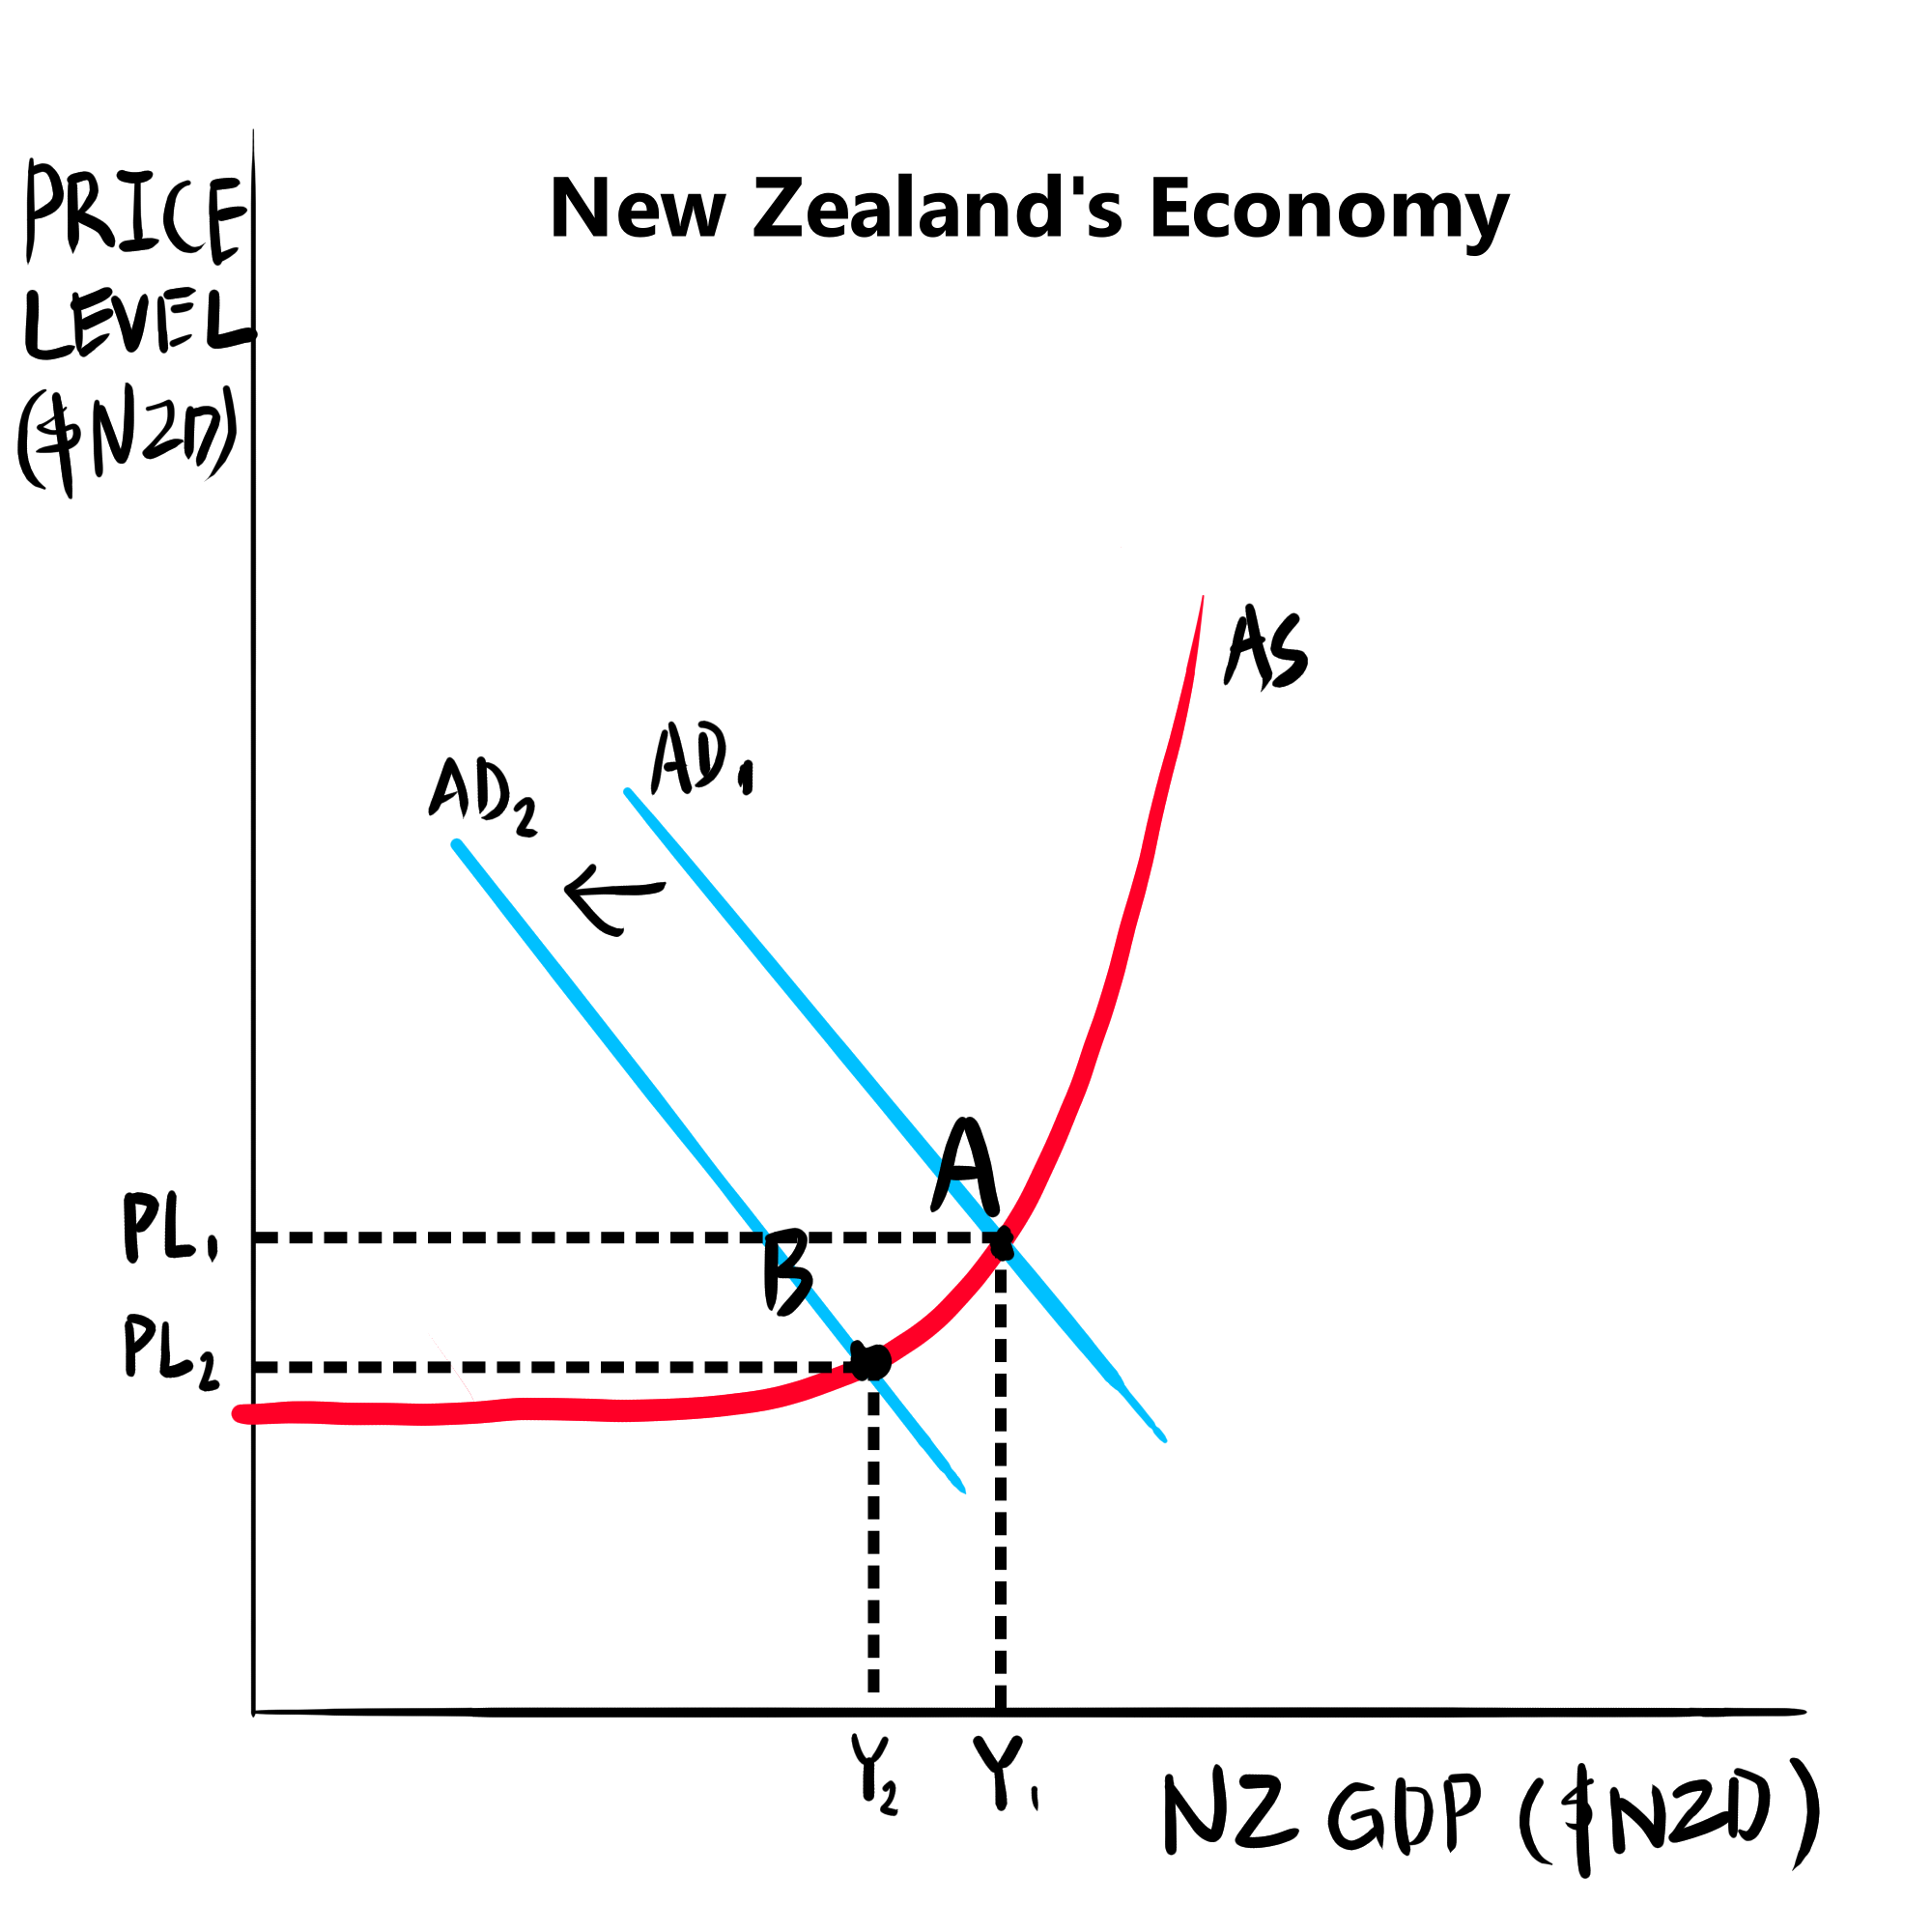
\includegraphics[width=0.6\textwidth]{assets/macro.png}
\end{figure}

Increased interest rates will decrease the amount of consumer spendings ($C$) and business investments ($I$) --- for it incentives savings and makes leveraging more expensive. Both are determinants of aggregate demand (AD) --- the total demands in an economy at various price levels. Therefore when $C$ and $I$ falls, AD will decrease and shift to the left from $AD_1$ to $AD_2$. Aggregate supply (AS) is the total supply of goods and services in an economy, and the Keysian model of AS is used because of NZ's strong labour unions creating downwards sticky wages \parencite{labor}. The fall in AD moves the equilibrium position from $A$ to $B$, decreasing NZ's real GDP from $Y_1$ to $Y_2$ and lowers the price level from $PL_1$ to $PL_2$, ceteris paribus. It looks like the policy is a step towards disinflation in New Zealand.
% TODO: do I need to explain the position of Y1 using unemployment statistics?

% connection to key concept
The concept of change is reflected in the change of approach against the pandemic. The article identified the OCR increase as one of the first deflationary intervention since the recession caused by the virus, this signifies a change in NZ's macroeconomic focus towards curbing inflation over economic growth. However, this creates some changes for various stakeholders.

% TODO: explain how it works? what does that mean

% evlauation of policy
The policy could affect certain households and firms and lower economic growth. The lower $AD$ will decrease national real output, and firm may lay-off inactive workers to counteract lower aggregate demands. But NZ's strong labour protection laws means that firms in the short-run will be unable to fire workers, needing to absorb the inefficiency and potentially creating losses in manufacturing sectors; Debter and home-buyers --- which are predominately young workers, will be paying more in loan interests and have less disposable income. This could largely reducing demand for goods \& services for the workers often have a high propensity of consumption, which justifies the large decrease in $AD$ and will lower short-term economic growth. Furthermore, this change is likely to increase wealth inequality between poorer debters and wealthier loaners, and may lower workers' health and education from lower disposable income, which may reduce potential productivity over-time and decrease long-run economic growth, restricting the pandemic recovery.

%The higher interest rates only makes paying this debt more expensive, further increasing the cost for firms forcing them to layoff workers, creating a spiral of higher costs and laying off workers. This serves to increase unemployment rate and lower household income in the long term --- due to the interdependence between households and firms. This may majorly affect the poorer populations and increase inequality if the spiral persists.
%Additionally, the policy may overshoot in disinflating the economy, causing deflation that further damages firms in increasing the relative costs of debt.

But the consequences can be reduced through gradual changes of the interest rate. Gradual interest rates increases allows the economy to adjust, and a slow decrease in fiscal benefits gives the incentives for labours to accept lower wages. This may reduce the problem of sticky wages, with the NZ economy having an inelastic long-run aggregate supply:

\begin{figure}[H]
    \centering
    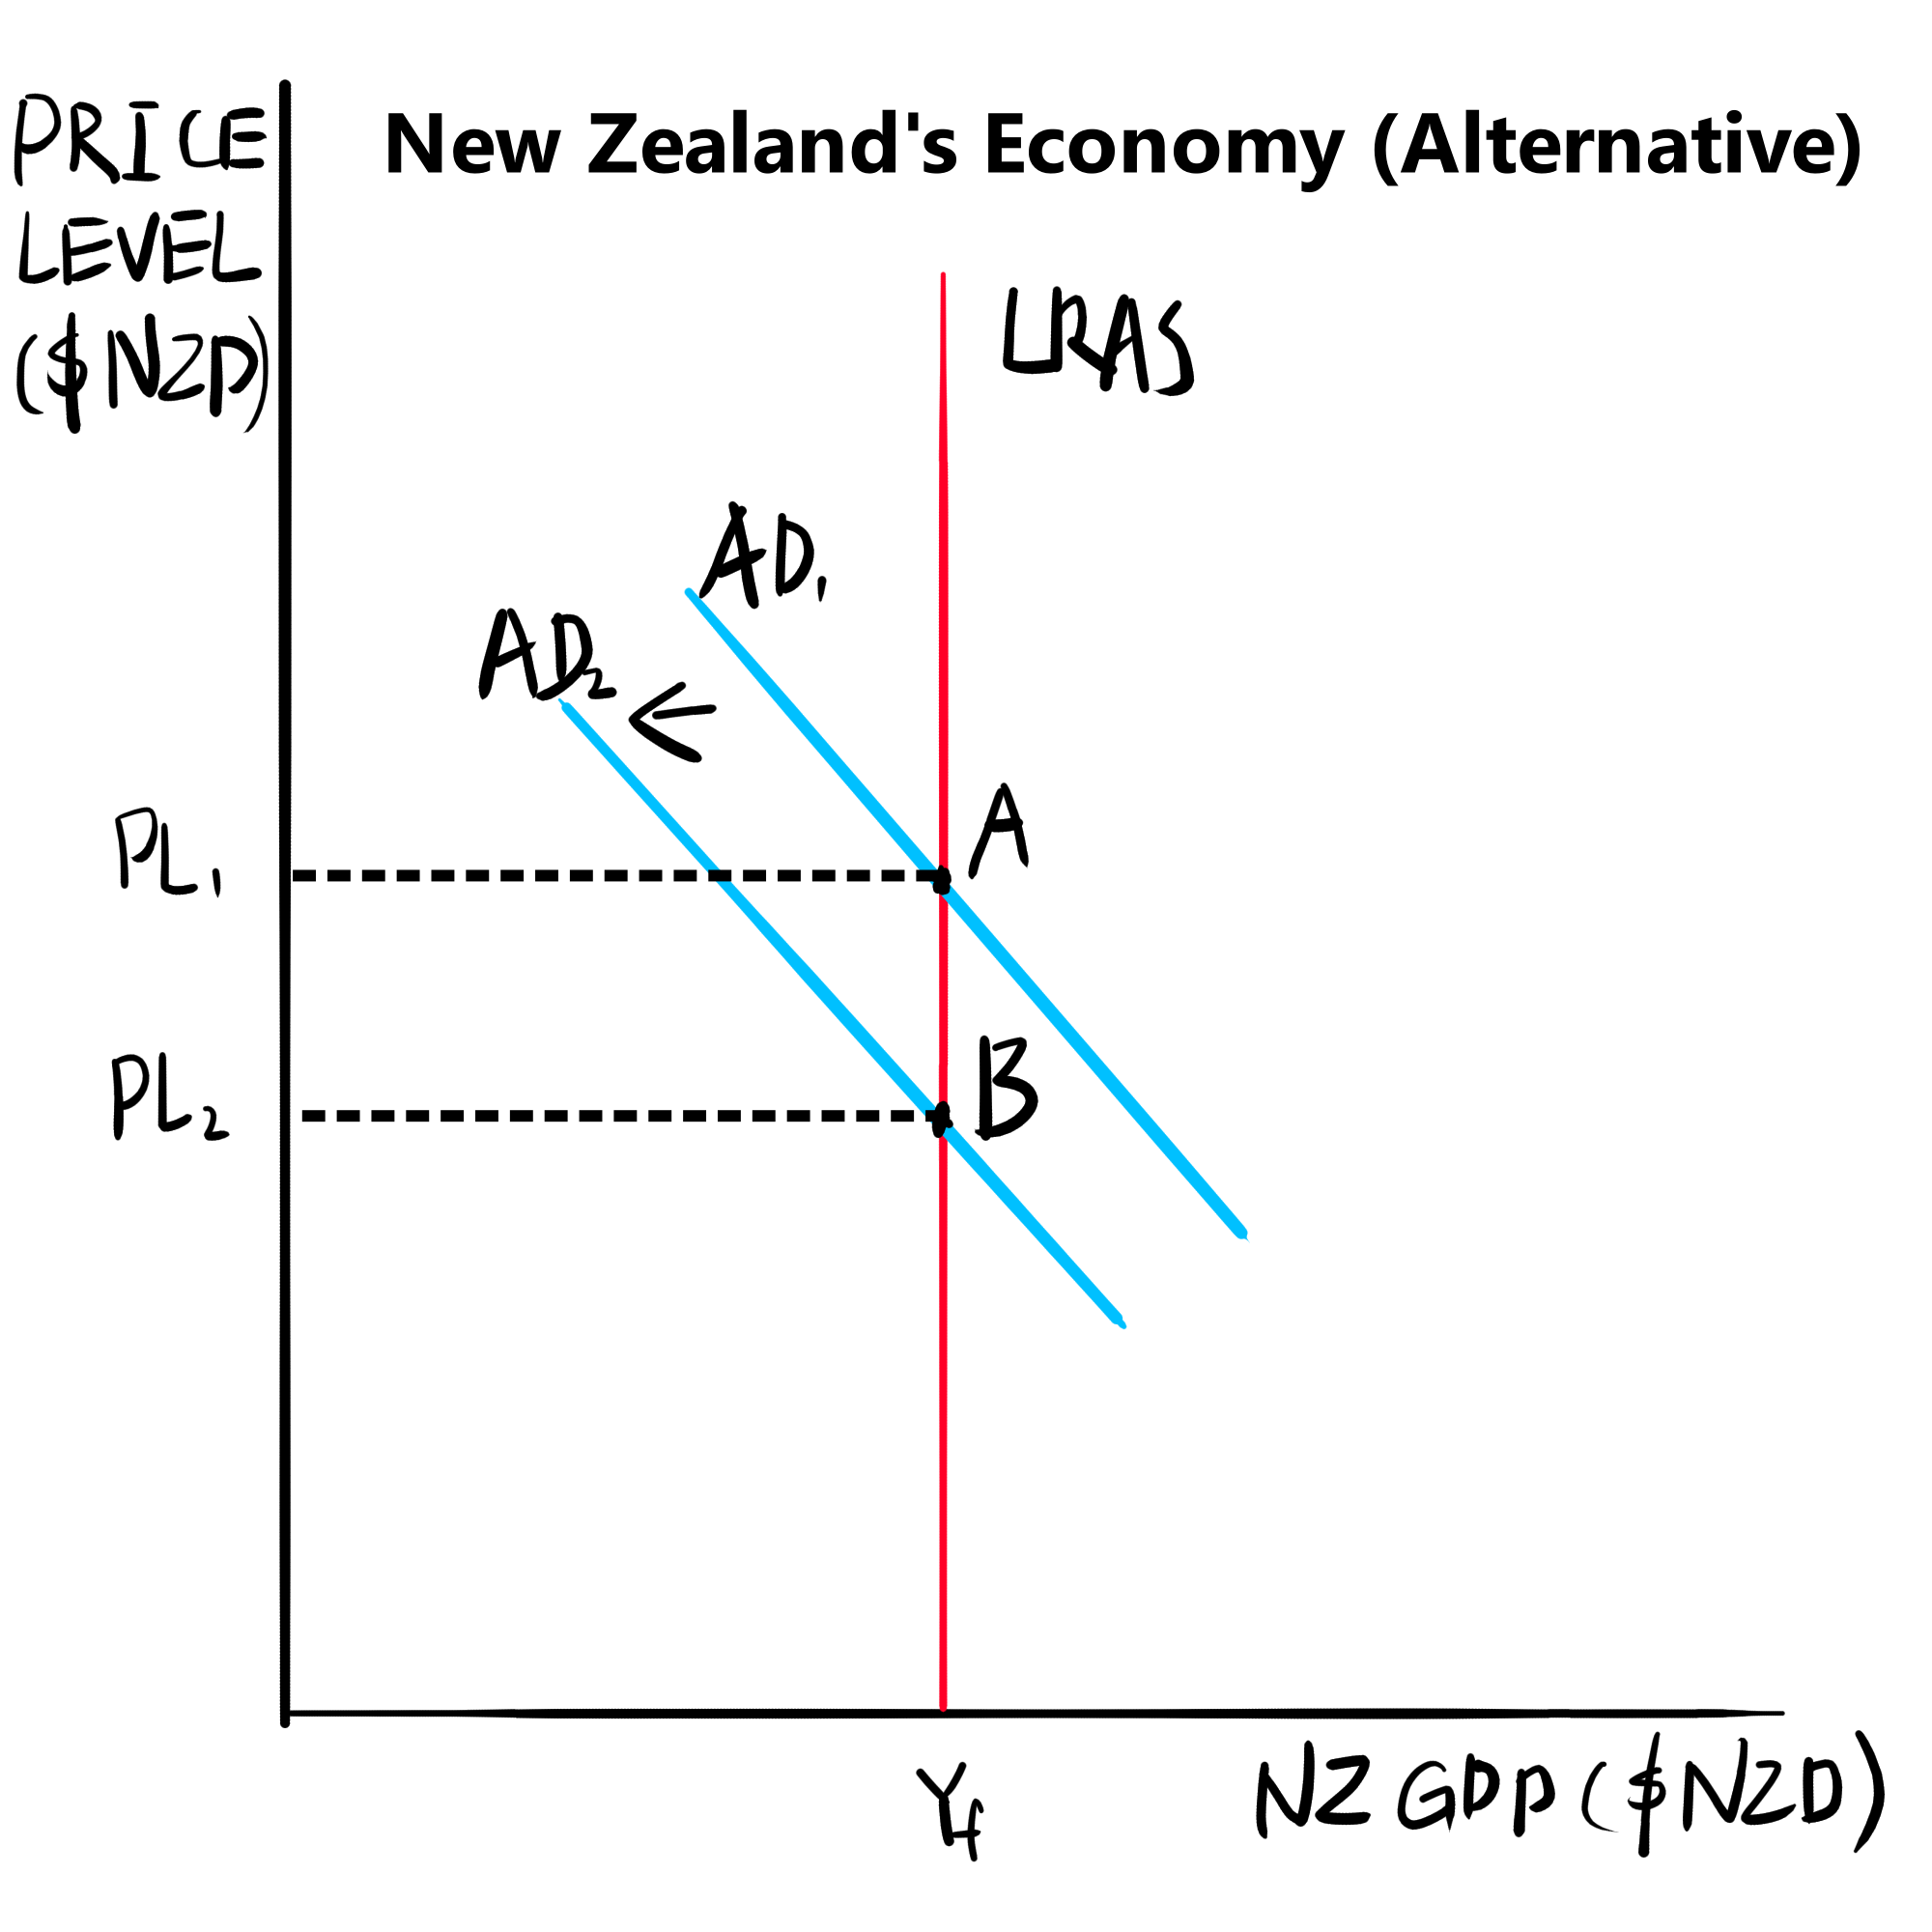
\includegraphics[width=0.6\textwidth]{assets/macro_alt.png}
\end{figure}

The decrease in $AD$ from $AD_1$ to $AD_2$ will only be deflationary in the long run as the workers --- owners of factors of productions, are willing to take lower wages at a recessionary gap when the economy moves from $A$ to $B$, decreasing short-run cost of productions and shifting $SRAS$ downwards from $SRAS_1$ to $SRAS_2$. The equilibrium position then moves from $B$ to $C$, decreasing the price level from $PL_1$ to $PL_3$ overall without affecting long run real GDP ($Y_f$). Additionally, the disinflation helps with confidence, raising consumption and investments by firms in the long-run, creating economic growth.

However, even gradual changes may not be without consequences. The increased interest rates will attract foreign investors and increase the demand of the New Zealand Dollar (NZD) on the foreign exchange market. This is likely to lead to an appreciation of NZD, which will reduce NZ's export competitiveness as it becomes relatively more expensive for foreign consumers to purchase its exports; and will also decrease the cost of imported products, increase the trade deficit. Also, the gradual change means the price elasticity of imports and exports are elastic so export revenue falls and import expenditure increases. As NZ is a large exporting economy \parencite{exports}, the policy is likely to hurt a lot of domestic firms mainly in the dairy and seafood industry, who are now forced to compete with cheaper foreign imports and may receive lower revenues. This would affect business confidence and decreases economic recovery in the short-run.

Although increasing OCR is an efficient method of disinflation, its consequences need to be monitored and cared for.

%But even gradual changes in the interest rate will structurally change the NZ housing market. Higher borrowing costs will increase the cost of a first home for home buyers in the short and long term, as national banks began delegating the increased interest rate to buyers in higher mortgage costs. For housing are necessities, living costs will increase particularly for young first home buyers.


% alternatives

% conclusion
\newpage
\printbibliography


\end{document}
